Applikationen har 3 forskellige aktører, 2 primære og 1 sekunder, som kan ses herunder på figur \ref{fig:aktor_konteks}.
\begin{figure}[h]
  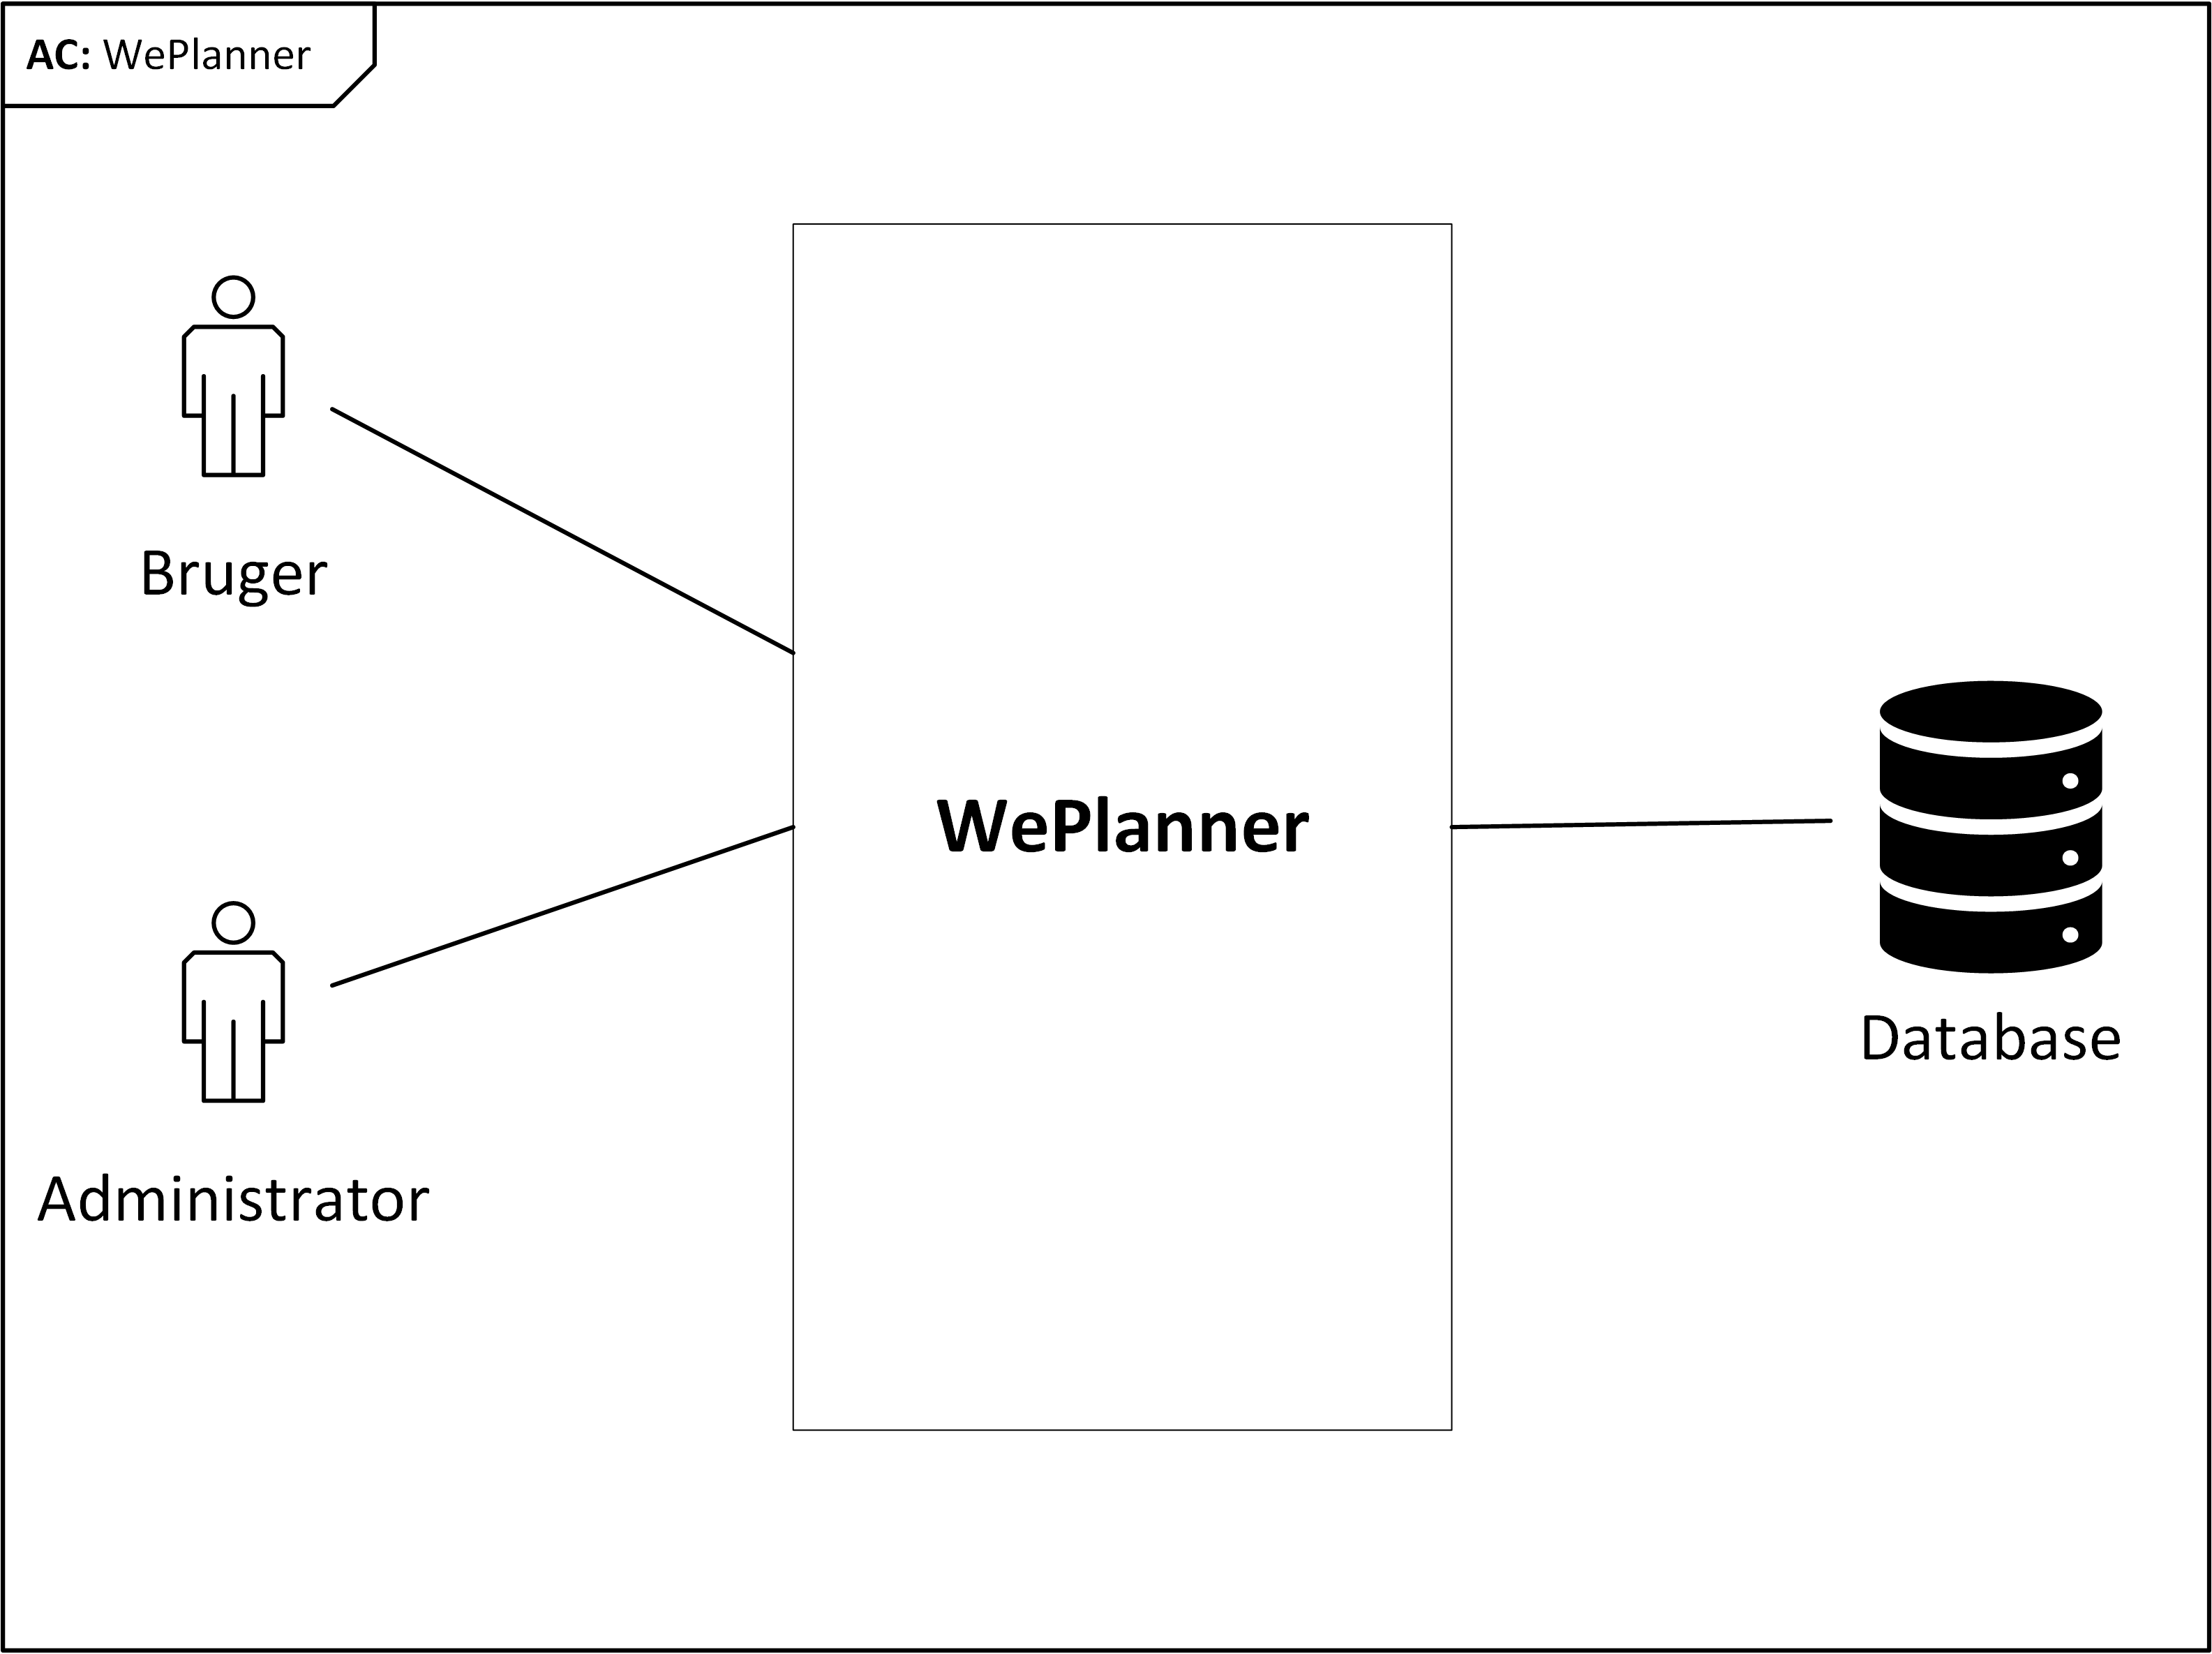
\includegraphics[width=\linewidth]{Kravspecifikation/Images/Aktor-kontekst_diagram.png}
  \caption{Aktør-kontekst diagram}
  \label{fig:aktor_konteks}
\end{figure}

\subsection{Bruger:}
Aktøren bruger er en person som har oprettet et brugerlogin til WePlanner, og dermed kan logge sig ind på siden. En bruger kan være en del af et eller flere bofællesskaber, og bliver en del af et sådant fællesskab, enten ved selv at oprette et fællesskab, eller ved at blive inviteret til et. Når en bruger er en del af fællesskabet kan brugeren se og oprette widgets på siden, som alle medlemmer af gruppen er en del af. 

\subsection{Administrator:}
I hvert bofællesskab vil der være en eller flere administratorer. Brugeren som opretter et bofællesskab vil automatisk blive administrator. En administrator kan derefter ophøje et andet medlem af gruppens rettigheder til administratorrettigheder. \\
En administrator har rettighed til at smide brugere ud af et bofællesskab, samt slette oprettede widgets.

\subsection{Database:}
Databasen er SQL-baseret, og indeholder informationerne for alle brugere og bofællesskaber. Det er her der bliver gemt loginoplysninger for brugere, og også her alle widgets for de individuelle bofællesskaber vil blive gemt. Databasen vil ligge online.